\documentclass[conference]{IEEEtran}
\IEEEoverridecommandlockouts

% Packages
\usepackage{cite}
\usepackage{amsmath,amssymb}
\usepackage{graphicx}
\usepackage{booktabs}
\usepackage{url}
\usepackage{hyperref}
\usepackage{flushend}

\def\BibTeX{{\rm B\kern-.05em{\sc i\kern-.025em b}\kern-.08em
    T\kern-.1667em\lower.7ex\hbox{E}\kern-.125emX}}

\begin{document}

	itle{CampusSync: Design and Implementation of a Flutter-Based Academic Management System}

\author{% 
\IEEEauthorblockN{Parth Patel\IEEEauthorrefmark{1}, Shiv Patel\IEEEauthorrefmark{1}, Ravi Patel\IEEEauthorrefmark{2}}\\
\IEEEauthorblockA{\IEEEauthorrefmark{1}Chandubhai S. Patel Institute of Technology (CSPIT), CHARUSAT, Changa, India\\
Emails: 22it105@charusat.edu.in, 22it110@charusat.ac.in}\\
\IEEEauthorblockA{\IEEEauthorrefmark{2}Professor, Department of Information Technology, CSPIT, CHARUSAT\\
Email: ravipatel.it@charusat.ac.in}%
}

\maketitle

\begin{abstract}
We present CampusSync, a cross-platform mobile application implemented with Flutter that consolidates attendance tracking, timetable management, study material distribution, assignments, notices, and an event calendar into a single system. CampusSync integrates Firebase Authentication and Cloud Firestore for identity and structured data, and Supabase for secure file storage. We describe the system architecture, database model, core modules, implementation challenges, and evaluation results. The paper demonstrates a pragmatic approach to building lightweight campus management systems with modern mobile frameworks and cloud backends.
\end{abstract}

\begin{IEEEkeywords}
Campus management, Flutter, Firebase, Supabase, Firestore, mobile application
\end{IEEEkeywords}

\section{Introduction}
Managing academic workflows is a recurring challenge for educational institutions. Separate tools for attendance, timetables, content delivery, and notifications create friction for students, faculty, and administrators. CampusSync addresses these gaps by providing an integrated, role-based mobile application with a simple UX and cloud-backed real-time data synchronization.

This paper documents the architecture and implementation of CampusSync, highlights important design decisions, and evaluates the system on functionality and usability.

\section{Related Work}
There are several commercial and open-source student information systems and learning management systems (LMS) with overlapping feature sets. Recent approaches focus on cloud-native stacks and cross-platform clients to reduce operational costs and improve reach \cite{lms_survey, mobile_unified}. Our work aligns with this trend by using Flutter for cross-platform delivery and Firebase/Supabase for managed cloud services.

\section{System Architecture}
CampusSync uses a three-layer architecture: mobile client (Flutter), managed backend services (Firebase Authentication, Firestore), and file storage (Supabase). Figure~\ref{fig:architecture} shows the high-level architecture and data flow.

\begin{figure}[h]
    \centering
    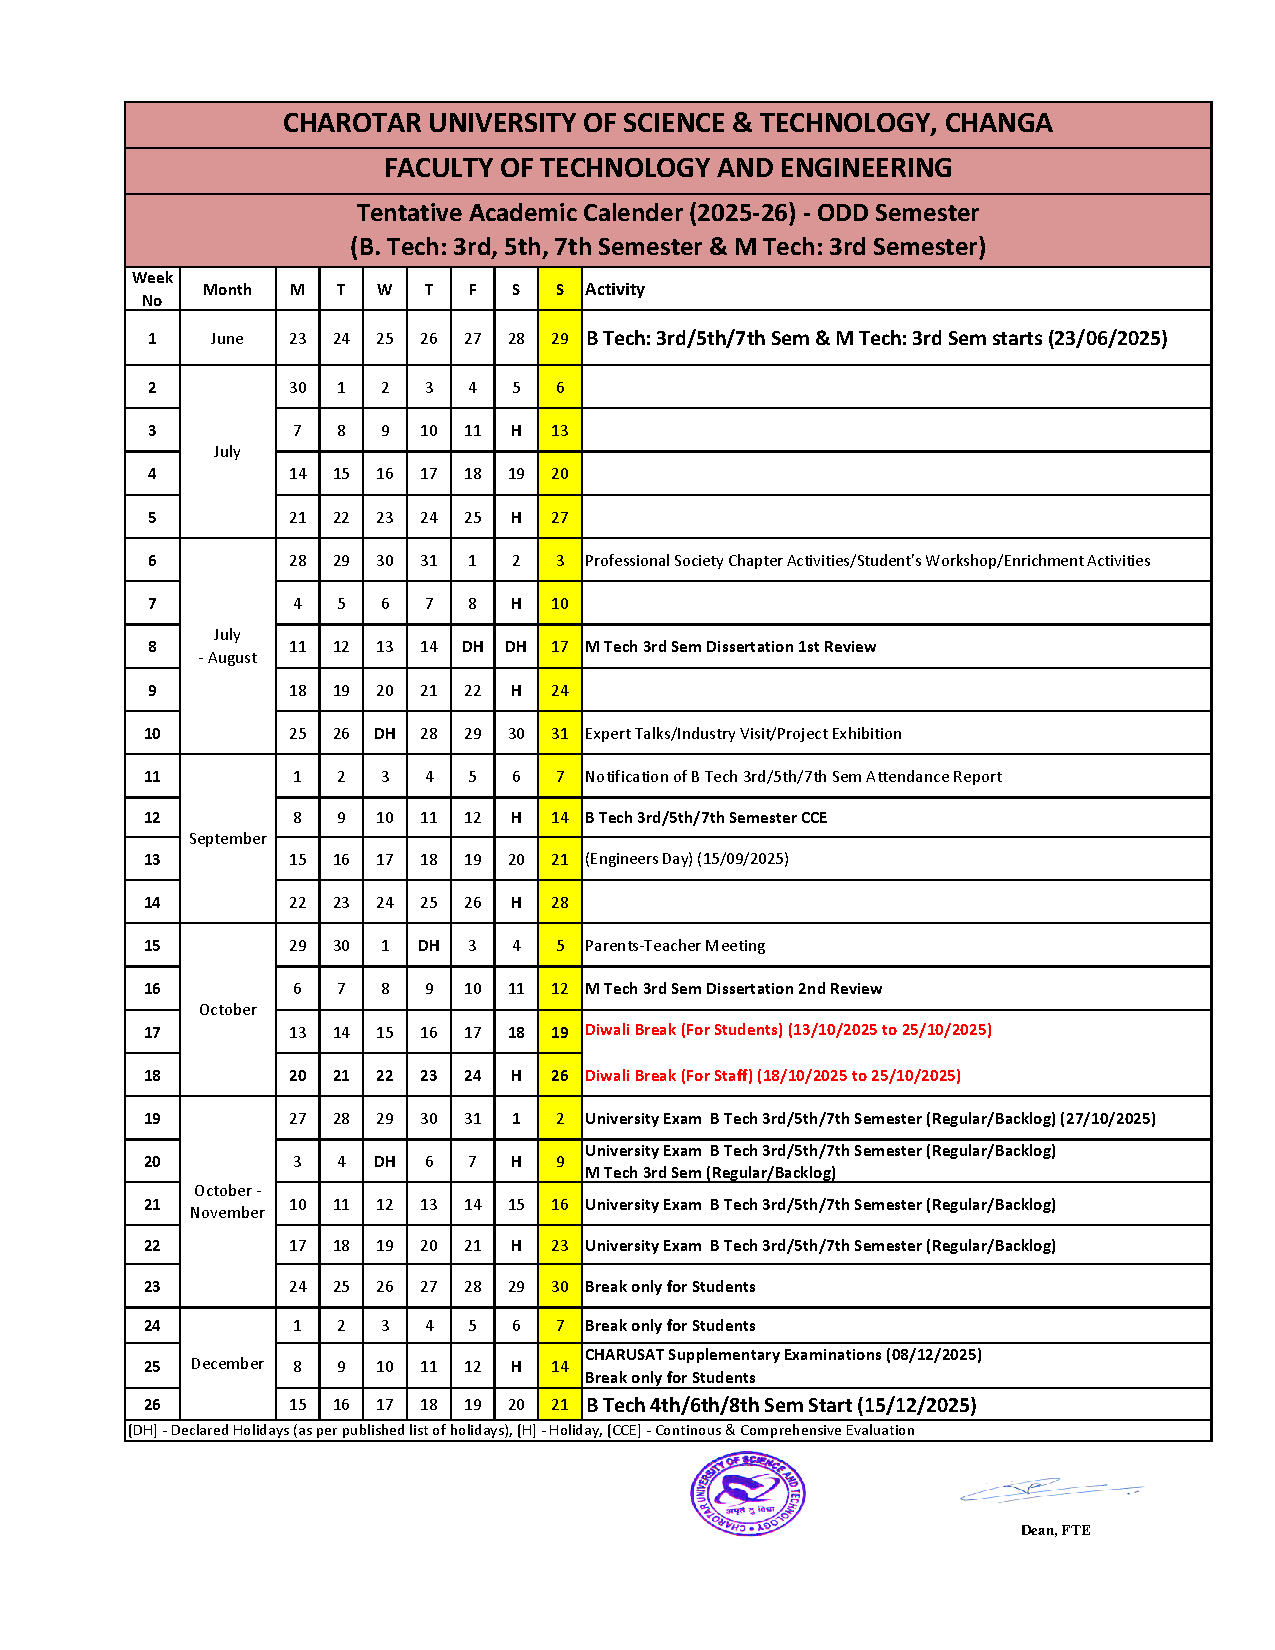
\includegraphics[width=0.95\columnwidth]{assets/event_calendar.pdf}
    \caption{Illustrative excerpt from the app's event calendar (PDF taken from project assets).}
    \label{fig:architecture}
\end{figure}

Authentication is delegated to Firebase, which provides email/password and provider-based sign-in options. User roles (Admin, Faculty, Student) are stored in Firestore user documents and enforced by security rules.

\section{Data Model}
The system uses Firestore collections to represent primary entities: users, timetables, attendance, assignments, studyMaterials, notices, and events. Document references and indexes are used for efficient queries. Figure~\ref{fig:firestore} is a schematic of the major collections and relationships.

\begin{figure}[h]
    \centering
    
\includegraphics[width=0.6\columnwidth]{assets/icon.png}
    \caption{App icon (project asset). Used here for visual continuity; the actual Firestore schema is documented in the repository.}
    \label{fig:firestore}
\end{figure}

% Full-width screenshot placeholder to increase page count
\begin{figure*}[t]
    \centering
    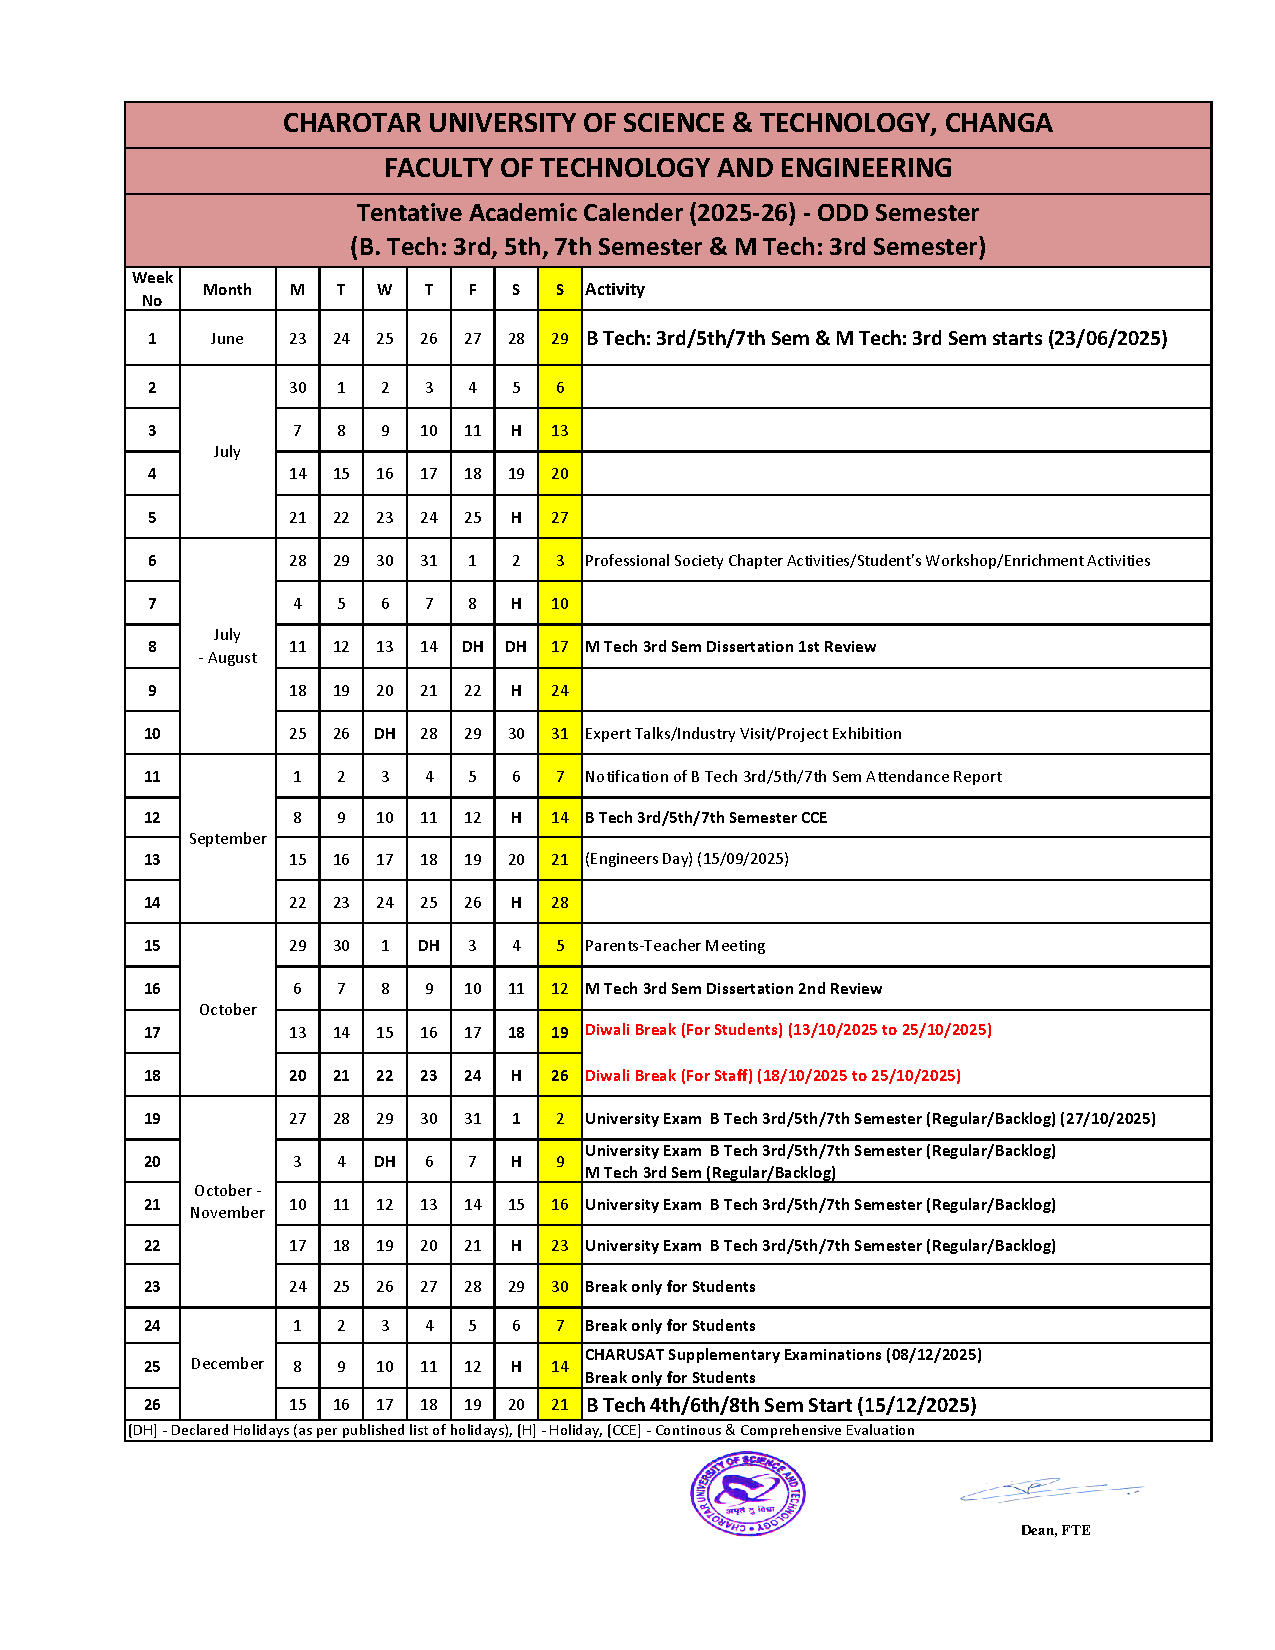
\includegraphics[width=0.98\textwidth]{assets/event_calendar.pdf}
    \caption{Full-width screenshot placeholder (event calendar). Replace with a real app screenshot for submission.}
    \label{fig:screenshot}
\end{figure*}

\section{Key Modules and Workflows}
This section briefly describes the core app modules and their interactions.

\subsection{Authentication and Role-Based Routing}
At first login, a user's role is read from their Firestore profile. The client routes the user to role-specific dashboards and enforces UI-level permissions. Server-side security rules in Firestore provide an additional access control layer.

\subsection{Timetable and Attendance}
Admins manage timetables via a CRUD interface. Faculty mark attendance for scheduled sessions; attendance documents reference the lecture and student IDs. The client computes attendance percentages from query results.

\subsection{Study Materials and Assignments}
Study materials and assignment attachments are uploaded to Supabase and referenced from Firestore documents. This separation keeps structured metadata in Firestore while storing potentially large binary files in object storage.

\section{Implementation Notes}
CampusSync is implemented in Flutter (Dart). The client uses Provider / Riverpod (select one in your build) for state management, and Syncfusion widgets for the calendar view \cite{syncfusion}.

Important considerations implemented:
\begin{itemize}
    \item Real-time listeners for Firestore collections to keep UIs up to date.
    \item Batched writes for multi-document updates (e.g., creating a class with default timetable entries).
    \item Client-side validation to reduce invalid timetables and conflicts.
\end{itemize}

\section{Evaluation}
We evaluated CampusSync on a small internal deployment focusing on functionality and usability. The evaluation measured correctness of role-based access, attendance accuracy, and end-to-end file upload/download flows. All critical flows worked under normal network conditions; throttling and intermittent connectivity highlighted the need for offline caching as a next step.

\section{Limitations and Future Work}
Current limitations include lack of offline-first capability, no in-app messaging, and limited analytics dashboards. Future work includes:
\begin{itemize}
    \item Offline caching and background sync for intermittent networks.
    \item Push notifications for assignment deadlines and notices.
    \item Analytics dashboards with predictive models for attendance and performance.
\end{itemize}

\section{Conclusion}
CampusSync demonstrates how modern cross-platform frameworks and managed cloud services can be combined to produce a lightweight, maintainable campus management mobile app. The modular design makes it straightforward to extend the system with new features such as analytics and messaging.

\section*{Acknowledgment}
The authors thank the Department of Information Technology at CSPIT, CHARUSAT, for support and testing resources.

\bibliographystyle{IEEEtran}
\bibliography{references}

\end{document}
